% Options for packages loaded elsewhere
\PassOptionsToPackage{unicode}{hyperref}
\PassOptionsToPackage{hyphens}{url}
\PassOptionsToPackage{dvipsnames,svgnames,x11names}{xcolor}
%
\documentclass[
  letterpaper,
  DIV=11,
  numbers=noendperiod]{scrartcl}

\usepackage{amsmath,amssymb}
\usepackage{iftex}
\ifPDFTeX
  \usepackage[T1]{fontenc}
  \usepackage[utf8]{inputenc}
  \usepackage{textcomp} % provide euro and other symbols
\else % if luatex or xetex
  \usepackage{unicode-math}
  \defaultfontfeatures{Scale=MatchLowercase}
  \defaultfontfeatures[\rmfamily]{Ligatures=TeX,Scale=1}
\fi
\usepackage{lmodern}
\ifPDFTeX\else  
    % xetex/luatex font selection
\fi
% Use upquote if available, for straight quotes in verbatim environments
\IfFileExists{upquote.sty}{\usepackage{upquote}}{}
\IfFileExists{microtype.sty}{% use microtype if available
  \usepackage[]{microtype}
  \UseMicrotypeSet[protrusion]{basicmath} % disable protrusion for tt fonts
}{}
\makeatletter
\@ifundefined{KOMAClassName}{% if non-KOMA class
  \IfFileExists{parskip.sty}{%
    \usepackage{parskip}
  }{% else
    \setlength{\parindent}{0pt}
    \setlength{\parskip}{6pt plus 2pt minus 1pt}}
}{% if KOMA class
  \KOMAoptions{parskip=half}}
\makeatother
\usepackage{xcolor}
\setlength{\emergencystretch}{3em} % prevent overfull lines
\setcounter{secnumdepth}{-\maxdimen} % remove section numbering
% Make \paragraph and \subparagraph free-standing
\ifx\paragraph\undefined\else
  \let\oldparagraph\paragraph
  \renewcommand{\paragraph}[1]{\oldparagraph{#1}\mbox{}}
\fi
\ifx\subparagraph\undefined\else
  \let\oldsubparagraph\subparagraph
  \renewcommand{\subparagraph}[1]{\oldsubparagraph{#1}\mbox{}}
\fi

\usepackage{color}
\usepackage{fancyvrb}
\newcommand{\VerbBar}{|}
\newcommand{\VERB}{\Verb[commandchars=\\\{\}]}
\DefineVerbatimEnvironment{Highlighting}{Verbatim}{commandchars=\\\{\}}
% Add ',fontsize=\small' for more characters per line
\usepackage{framed}
\definecolor{shadecolor}{RGB}{241,243,245}
\newenvironment{Shaded}{\begin{snugshade}}{\end{snugshade}}
\newcommand{\AlertTok}[1]{\textcolor[rgb]{0.68,0.00,0.00}{#1}}
\newcommand{\AnnotationTok}[1]{\textcolor[rgb]{0.37,0.37,0.37}{#1}}
\newcommand{\AttributeTok}[1]{\textcolor[rgb]{0.40,0.45,0.13}{#1}}
\newcommand{\BaseNTok}[1]{\textcolor[rgb]{0.68,0.00,0.00}{#1}}
\newcommand{\BuiltInTok}[1]{\textcolor[rgb]{0.00,0.23,0.31}{#1}}
\newcommand{\CharTok}[1]{\textcolor[rgb]{0.13,0.47,0.30}{#1}}
\newcommand{\CommentTok}[1]{\textcolor[rgb]{0.37,0.37,0.37}{#1}}
\newcommand{\CommentVarTok}[1]{\textcolor[rgb]{0.37,0.37,0.37}{\textit{#1}}}
\newcommand{\ConstantTok}[1]{\textcolor[rgb]{0.56,0.35,0.01}{#1}}
\newcommand{\ControlFlowTok}[1]{\textcolor[rgb]{0.00,0.23,0.31}{#1}}
\newcommand{\DataTypeTok}[1]{\textcolor[rgb]{0.68,0.00,0.00}{#1}}
\newcommand{\DecValTok}[1]{\textcolor[rgb]{0.68,0.00,0.00}{#1}}
\newcommand{\DocumentationTok}[1]{\textcolor[rgb]{0.37,0.37,0.37}{\textit{#1}}}
\newcommand{\ErrorTok}[1]{\textcolor[rgb]{0.68,0.00,0.00}{#1}}
\newcommand{\ExtensionTok}[1]{\textcolor[rgb]{0.00,0.23,0.31}{#1}}
\newcommand{\FloatTok}[1]{\textcolor[rgb]{0.68,0.00,0.00}{#1}}
\newcommand{\FunctionTok}[1]{\textcolor[rgb]{0.28,0.35,0.67}{#1}}
\newcommand{\ImportTok}[1]{\textcolor[rgb]{0.00,0.46,0.62}{#1}}
\newcommand{\InformationTok}[1]{\textcolor[rgb]{0.37,0.37,0.37}{#1}}
\newcommand{\KeywordTok}[1]{\textcolor[rgb]{0.00,0.23,0.31}{#1}}
\newcommand{\NormalTok}[1]{\textcolor[rgb]{0.00,0.23,0.31}{#1}}
\newcommand{\OperatorTok}[1]{\textcolor[rgb]{0.37,0.37,0.37}{#1}}
\newcommand{\OtherTok}[1]{\textcolor[rgb]{0.00,0.23,0.31}{#1}}
\newcommand{\PreprocessorTok}[1]{\textcolor[rgb]{0.68,0.00,0.00}{#1}}
\newcommand{\RegionMarkerTok}[1]{\textcolor[rgb]{0.00,0.23,0.31}{#1}}
\newcommand{\SpecialCharTok}[1]{\textcolor[rgb]{0.37,0.37,0.37}{#1}}
\newcommand{\SpecialStringTok}[1]{\textcolor[rgb]{0.13,0.47,0.30}{#1}}
\newcommand{\StringTok}[1]{\textcolor[rgb]{0.13,0.47,0.30}{#1}}
\newcommand{\VariableTok}[1]{\textcolor[rgb]{0.07,0.07,0.07}{#1}}
\newcommand{\VerbatimStringTok}[1]{\textcolor[rgb]{0.13,0.47,0.30}{#1}}
\newcommand{\WarningTok}[1]{\textcolor[rgb]{0.37,0.37,0.37}{\textit{#1}}}

\providecommand{\tightlist}{%
  \setlength{\itemsep}{0pt}\setlength{\parskip}{0pt}}\usepackage{longtable,booktabs,array}
\usepackage{calc} % for calculating minipage widths
% Correct order of tables after \paragraph or \subparagraph
\usepackage{etoolbox}
\makeatletter
\patchcmd\longtable{\par}{\if@noskipsec\mbox{}\fi\par}{}{}
\makeatother
% Allow footnotes in longtable head/foot
\IfFileExists{footnotehyper.sty}{\usepackage{footnotehyper}}{\usepackage{footnote}}
\makesavenoteenv{longtable}
\usepackage{graphicx}
\makeatletter
\def\maxwidth{\ifdim\Gin@nat@width>\linewidth\linewidth\else\Gin@nat@width\fi}
\def\maxheight{\ifdim\Gin@nat@height>\textheight\textheight\else\Gin@nat@height\fi}
\makeatother
% Scale images if necessary, so that they will not overflow the page
% margins by default, and it is still possible to overwrite the defaults
% using explicit options in \includegraphics[width, height, ...]{}
\setkeys{Gin}{width=\maxwidth,height=\maxheight,keepaspectratio}
% Set default figure placement to htbp
\makeatletter
\def\fps@figure{htbp}
\makeatother

\KOMAoption{captions}{tableheading}
\makeatletter
\makeatother
\makeatletter
\makeatother
\makeatletter
\@ifpackageloaded{caption}{}{\usepackage{caption}}
\AtBeginDocument{%
\ifdefined\contentsname
  \renewcommand*\contentsname{Table of contents}
\else
  \newcommand\contentsname{Table of contents}
\fi
\ifdefined\listfigurename
  \renewcommand*\listfigurename{List of Figures}
\else
  \newcommand\listfigurename{List of Figures}
\fi
\ifdefined\listtablename
  \renewcommand*\listtablename{List of Tables}
\else
  \newcommand\listtablename{List of Tables}
\fi
\ifdefined\figurename
  \renewcommand*\figurename{Figure}
\else
  \newcommand\figurename{Figure}
\fi
\ifdefined\tablename
  \renewcommand*\tablename{Table}
\else
  \newcommand\tablename{Table}
\fi
}
\@ifpackageloaded{float}{}{\usepackage{float}}
\floatstyle{ruled}
\@ifundefined{c@chapter}{\newfloat{codelisting}{h}{lop}}{\newfloat{codelisting}{h}{lop}[chapter]}
\floatname{codelisting}{Listing}
\newcommand*\listoflistings{\listof{codelisting}{List of Listings}}
\makeatother
\makeatletter
\@ifpackageloaded{caption}{}{\usepackage{caption}}
\@ifpackageloaded{subcaption}{}{\usepackage{subcaption}}
\makeatother
\makeatletter
\@ifpackageloaded{tcolorbox}{}{\usepackage[skins,breakable]{tcolorbox}}
\makeatother
\makeatletter
\@ifundefined{shadecolor}{\definecolor{shadecolor}{rgb}{.97, .97, .97}}
\makeatother
\makeatletter
\makeatother
\makeatletter
\makeatother
\ifLuaTeX
  \usepackage{selnolig}  % disable illegal ligatures
\fi
\IfFileExists{bookmark.sty}{\usepackage{bookmark}}{\usepackage{hyperref}}
\IfFileExists{xurl.sty}{\usepackage{xurl}}{} % add URL line breaks if available
\urlstyle{same} % disable monospaced font for URLs
\hypersetup{
  pdftitle={Introduction to Quarto},
  pdfauthor={Lifeng Ren},
  colorlinks=true,
  linkcolor={blue},
  filecolor={Maroon},
  citecolor={Blue},
  urlcolor={Blue},
  pdfcreator={LaTeX via pandoc}}

\title{Introduction to Quarto}
\author{Lifeng Ren}
\date{2023-09-13}

\begin{document}
\maketitle
\ifdefined\Shaded\renewenvironment{Shaded}{\begin{tcolorbox}[interior hidden, borderline west={3pt}{0pt}{shadecolor}, sharp corners, boxrule=0pt, enhanced, frame hidden, breakable]}{\end{tcolorbox}}\fi

\hypertarget{overview}{%
\subsection{Overview}\label{overview}}

\begin{itemize}
\tightlist
\item
  Today, I am going to go over a software called \texttt{Quarto} that is
  developed by the same team that developed \texttt{R\ Markdown}. As you
  can guess for now, they are very similar with slight difference.
\item
  In this session, I am hoping to go over:

  \begin{itemize}
  \tightlist
  \item
    What is \texttt{Quarto}, and why we should use it
  \item
    How to use \texttt{Quarto} to generate:

    \begin{itemize}
    \tightlist
    \item
      \texttt{HTML} documents
    \item
      \texttt{Reveal.js} slides
    \item
      Quarto website with \texttt{GitHub\ Pages}
    \end{itemize}
  \end{itemize}
\end{itemize}

\hypertarget{what-is-quarto}{%
\subsection{What is Quarto}\label{what-is-quarto}}

\begin{itemize}
\item
  Quarto is an open-source scientific and technical publishing system to
  create dynamic content with \texttt{Python}, \texttt{R},
  \texttt{Stata}, \texttt{Julia} with engines \texttt{Jupyter},
  \texttt{Knitr}, and \texttt{Observable}.
\item
  Just like \texttt{R\ Markdown}, \texttt{Quarto} uses \texttt{PanDoc}
  to convert \texttt{Markdown} to \texttt{LaTex}, \texttt{HTML},
  \texttt{PDF}, \texttt{Word}, etc.
\item
  In short: One document (\texttt{.qmd}), multiple languages, multiple
  outputs.
\end{itemize}

\hypertarget{why-quarto}{%
\subsection{Why Quarto?}\label{why-quarto}}

\begin{itemize}
\item
  To keep your code and document in one place and make it reproducible.
  Most importantly, to make it open-sourced and shareable.
\item
  What if I am already using \texttt{R\ Markdown}, do I need to switch?

  \begin{itemize}
  \tightlist
  \item
    Based on your needs. There are many discussions on this, and I am
    providing some blogs and articles that you can read to make your own
    decision.

    \begin{itemize}
    \tightlist
    \item
      \href{https://yihui.org/en/2022/04/quarto-r-markdown/}{With Quarto
      Coming, is R Markdown Going Away? No.}
    \item
      \href{https://www.njtierney.com/post/2022/04/11/rmd-to-qmd/}{Notes
      on Changing from Rmarkdown/Bookdown to Quarto}
    \end{itemize}
  \end{itemize}
\end{itemize}

\hypertarget{install-quarto}{%
\subsection{Install Quarto}\label{install-quarto}}

To play with \texttt{Quarto}, you should firstly download Quarto from
\href{https://quarto.org/docs/get-started/}{here}, install it, and
choose your favorite IDE to write \texttt{Quarto} documents. I am using
\texttt{VS\ Code} with \texttt{Quarto} extension installed to show the
demo today.

\begin{itemize}
\item
  If you are using \texttt{R\ Studio}, once you installed
  \texttt{Quarto}, you do not need any extra steps. Just restart your
  \texttt{R\ Studio} and you are good to go.
\item
  In the \texttt{VS\ Code} IDE, you need to install \texttt{Quarto}
  extension in the \texttt{Extensions} marketplace.

  
\includegraphics[width=0.5\textwidth,height=\textheight]{img/quarto_extension.png}
\end{itemize}

\hypertarget{generate-your-first-quarto-document}{%
\section{\texorpdfstring{Generate your first \texttt{Quarto}
document}{Generate your first Quarto document}}\label{generate-your-first-quarto-document}}

As I mentioned above, \texttt{Quarto} can support many output formats.
Today, I am going to show you how to generate \texttt{HTML} documents,
\texttt{Reveal.js} slides, and \texttt{Quarto} website with
\texttt{GitHub\ Pages}. For a full list of reference, please visit this
page: \url{https://quarto.org/docs/guide/}.

\hypertarget{quarto-notebook}{%
\subsection{Quarto Notebook}\label{quarto-notebook}}

\begin{itemize}
\item
  Quarto provides a \texttt{Notebook\ Editor} and a
  \texttt{Visual\ Editor} mode to write the document. (DEMO)

  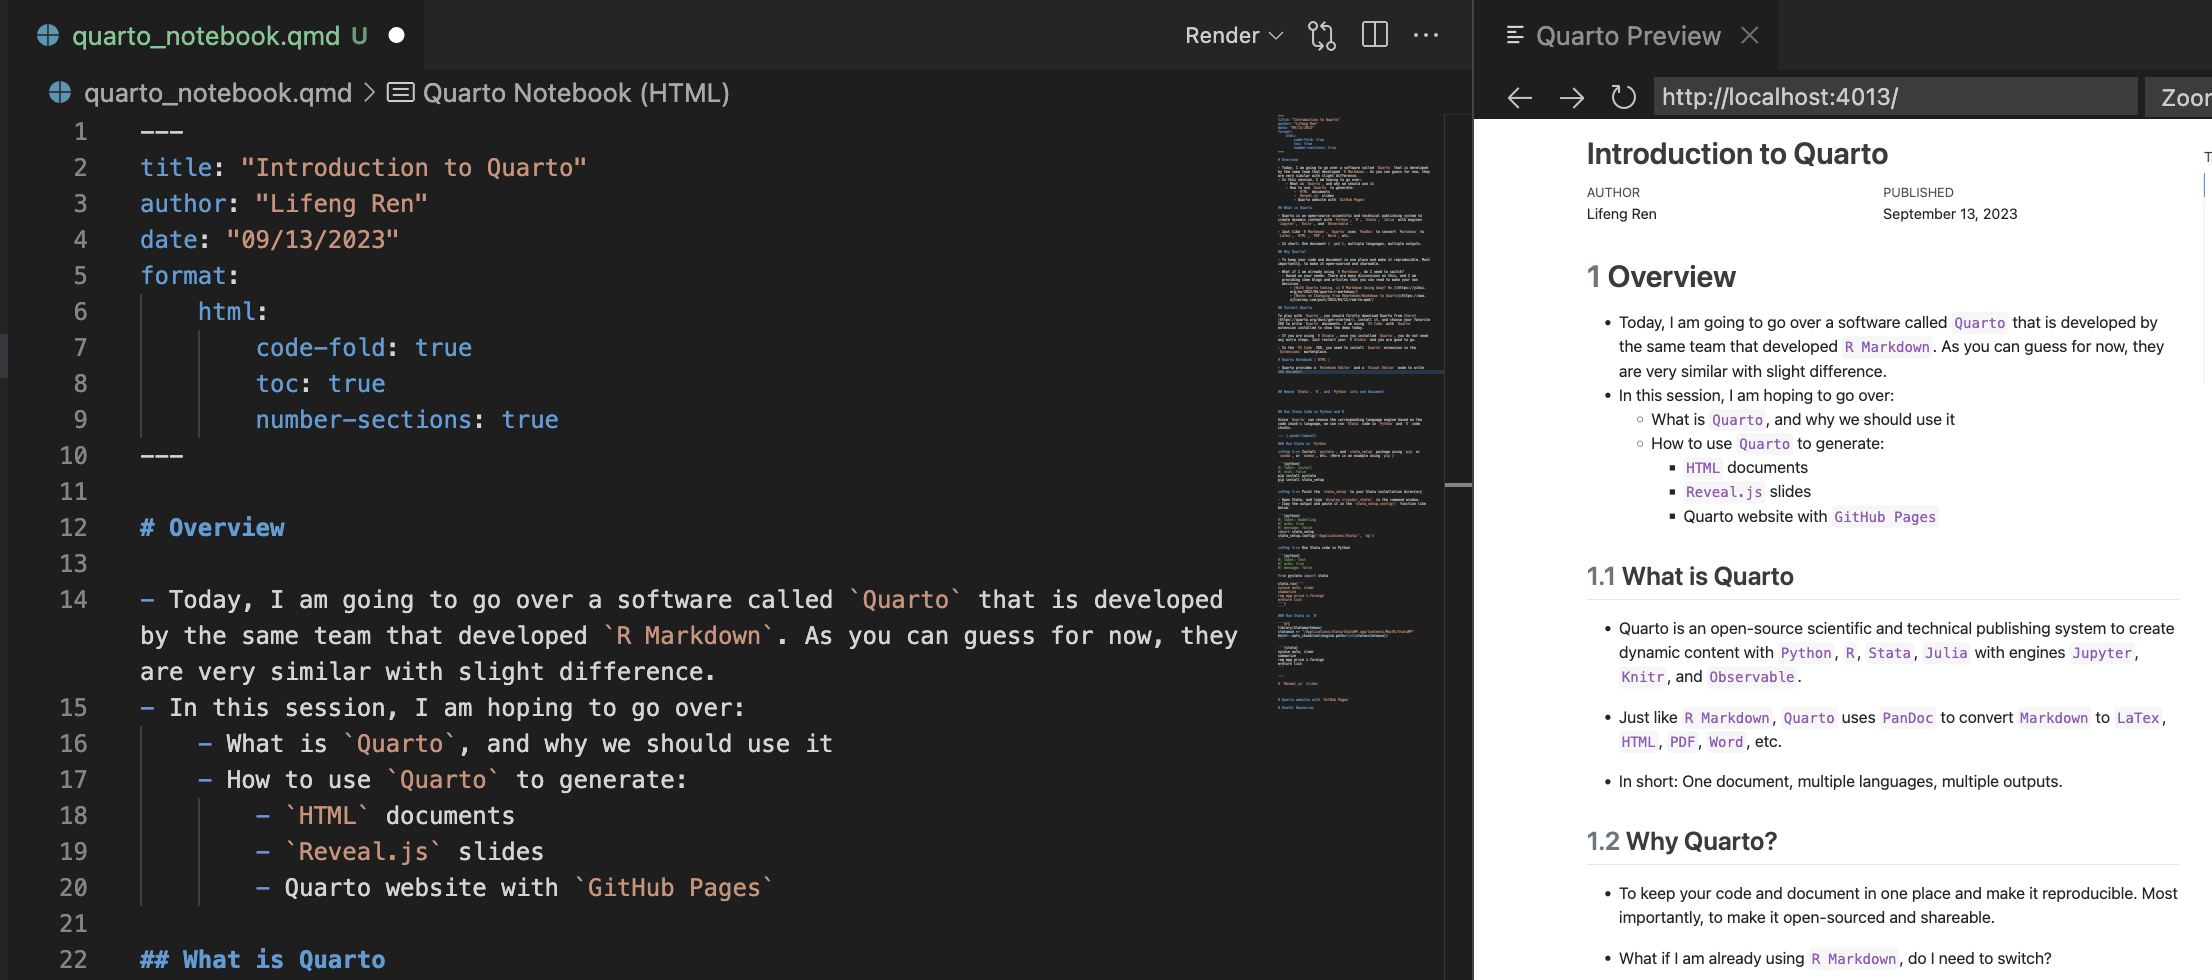
\includegraphics[width=0.5\textwidth,height=\textheight]{img/notebook_editor.png}
  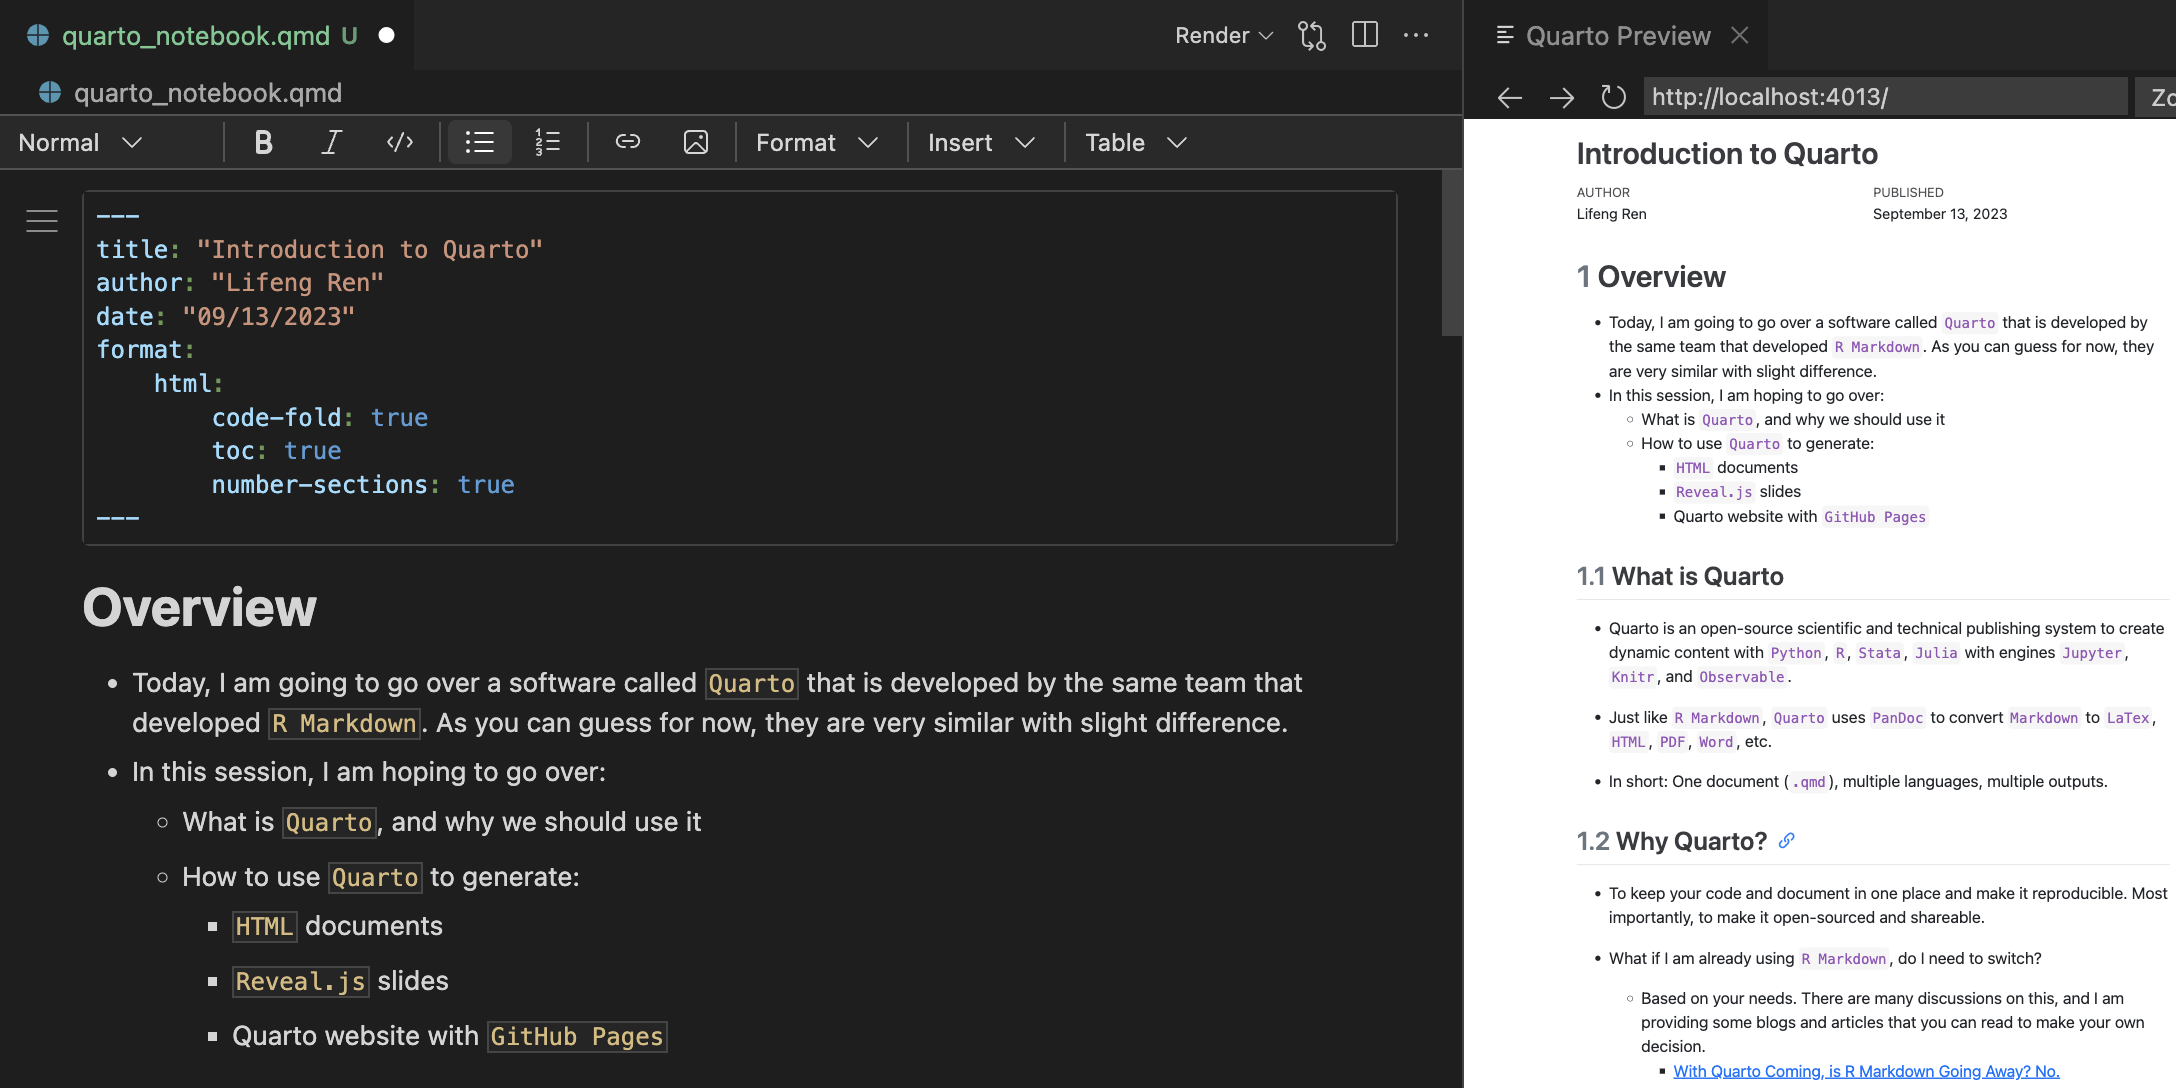
\includegraphics[width=0.5\textwidth,height=\textheight]{img/visual_editor.png}
\item
  It can be rendered into different type of outputs. (DEMO for
  \texttt{HTML}, \texttt{PDF}, \texttt{Word})

  \begin{itemize}
  \tightlist
  \item
    For now, I will keep rendering it into \texttt{HTML} format.
  \end{itemize}
\item
  Almost all syntax are the same for \texttt{R\ Markdown} and
  \texttt{Quarto} because they are based on \texttt{Markdown}. So, I
  won't go over the syntax a lot today. You can find more information
  here: \url{https://quarto.org/docs/authoring/markdown-basics.html}
\item
  \texttt{YAML} header has some differences. Here is an example:
\end{itemize}

\begin{longtable}[]{@{}
  >{\raggedright\arraybackslash}p{(\columnwidth - 2\tabcolsep) * \real{0.6429}}
  >{\raggedright\arraybackslash}p{(\columnwidth - 2\tabcolsep) * \real{0.3571}}@{}}
\toprule\noalign{}
\begin{minipage}[b]{\linewidth}\raggedright
RMarkdown
\end{minipage} & \begin{minipage}[b]{\linewidth}\raggedright
Quarto
\end{minipage} \\
\midrule\noalign{}
\endhead
\bottomrule\noalign{}
\endlastfoot
output: html\_document & format: html \\
output: pdf\_document & format: pdf \\
output: word\_document & format: docx \\
\texttt{underscore}: \texttt{\_} (e.g.:
\texttt{number\_sections:\ true}) & \texttt{dash}: \texttt{-} (e.g.:
\texttt{number-sections:\ true}) \\
Rerender all the code & Rerender only when source changes \\
\end{longtable}

New Features in \texttt{Quarto}'s \texttt{YAML} header:

\begin{Shaded}
\begin{Highlighting}[]
\NormalTok{execute}\SpecialCharTok{:}
\NormalTok{  freeze}\SpecialCharTok{:}\NormalTok{ auto  }\CommentTok{\# re{-}render only when source changes}
\end{Highlighting}
\end{Shaded}

\begin{itemize}
\tightlist
\item
  Code Chunk options are changing
\end{itemize}

\subsubsection{RMarkdown}

\begin{Shaded}
\begin{Highlighting}[]
    \StringTok{\textasciigrave{}\textasciigrave{}\textasciigrave{}}\AttributeTok{\{r setup, include=FALSE\}}
\AttributeTok{    }\StringTok{\textasciigrave{}\textasciigrave{}\textasciigrave{}}
\end{Highlighting}
\end{Shaded}

\subsubsection{Quarto}

\begin{Shaded}
\begin{Highlighting}[]
    \StringTok{\textasciigrave{}\textasciigrave{}\textasciigrave{}}\AttributeTok{\{r\}}
\AttributeTok{    \#| label: "setup"}
\AttributeTok{    \#| include: false}
\AttributeTok{    }\StringTok{\textasciigrave{}\textasciigrave{}\textasciigrave{}}
\end{Highlighting}
\end{Shaded}

\hypertarget{weave-stata-r-and-python-into-one-document}{%
\subsection{\texorpdfstring{Weave \texttt{Stata}, \texttt{R}, and
\texttt{Python} into one
Document}{Weave Stata, R, and Python into one Document}}\label{weave-stata-r-and-python-into-one-document}}

\hypertarget{run-stata-code-in-python-and-r}{%
\subsubsection{Run Stata Code in Python and
R}\label{run-stata-code-in-python-and-r}}

Since \texttt{Quarto} can choose the corresponding language engine based
on the code chunk's language, we can run \texttt{Stata} code in
\texttt{Python} and \texttt{R} code chunks to weave all three languages
coding into one document.

\paragraph{\texorpdfstring{Run Stata in
\texttt{Python}}{Run Stata in Python}}

\textbf{Step 1:} Install \texttt{pystata}, and \texttt{stata\_setup}
package using \texttt{pip} or \texttt{conda}, or \texttt{mamba}, etc.
(Here is an example using \texttt{pip})

\begin{Shaded}
\begin{Highlighting}[]
\NormalTok{pip install pystata}
\NormalTok{pip install stata\_setup}
\end{Highlighting}
\end{Shaded}

\textbf{Step 2:} Point the \texttt{stata\_setup} to your Stata
installation directory

\begin{itemize}
\tightlist
\item
  Open Stata, and type \texttt{display\ c(sysdir\_stata)} in the command
  window.
\item
  Copy the output and paste it in the \texttt{stata\_setup.config()}
  function like below.
\end{itemize}

\begin{Shaded}
\begin{Highlighting}[numbers=left,,]
\ImportTok{import}\NormalTok{ stata\_setup}
\NormalTok{stata\_setup.config(}\StringTok{\textquotesingle{}/Applications/Stata/\textquotesingle{}}\NormalTok{, }\StringTok{\textquotesingle{}mp\textquotesingle{}}\NormalTok{)}
\end{Highlighting}
\end{Shaded}

\begin{verbatim}

  ___  ____  ____  ____  ____ ®
 /__    /   ____/   /   ____/      17.0
___/   /   /___/   /   /___/       MP—Parallel Edition

 Statistics and Data Science       Copyright 1985-2021 StataCorp LLC
                                   StataCorp
                                   4905 Lakeway Drive
                                   College Station, Texas 77845 USA
                                   800-STATA-PC        https://www.stata.com
                                   979-696-4600        stata@stata.com

Stata license: Single-user 8-core , expiring  1 Jan 2025
Serial number: 501709301094
  Licensed to: Lifeng Ren
               APEC

Notes:
      1. Unicode is supported; see help unicode_advice.
      2. More than 2 billion observations are allowed; see help obs_advice.
      3. Maximum number of variables is set to 5,000; see help set_maxvar.
\end{verbatim}

\textbf{Step 3:} Run Stata code in Python

\begin{Shaded}
\begin{Highlighting}[]
\ImportTok{from}\NormalTok{ pystata }\ImportTok{import}\NormalTok{ stata}

\NormalTok{stata.run(}\StringTok{\textquotesingle{}\textquotesingle{}\textquotesingle{}}
\StringTok{sysuse auto, clear}
\StringTok{summarize}
\StringTok{reg mpg price i.foreign}
\StringTok{ereturn list}
\StringTok{\textquotesingle{}\textquotesingle{}\textquotesingle{}}\NormalTok{)}
\end{Highlighting}
\end{Shaded}

\begin{verbatim}

. 
. sysuse auto, clear
(1978 automobile data)

. summarize

    Variable |        Obs        Mean    Std. dev.       Min        Max
-------------+---------------------------------------------------------
        make |          0
       price |         74    6165.257    2949.496       3291      15906
         mpg |         74     21.2973    5.785503         12         41
       rep78 |         69    3.405797    .9899323          1          5
    headroom |         74    2.993243    .8459948        1.5          5
-------------+---------------------------------------------------------
       trunk |         74    13.75676    4.277404          5         23
      weight |         74    3019.459    777.1936       1760       4840
      length |         74    187.9324    22.26634        142        233
        turn |         74    39.64865    4.399354         31         51
displacement |         74    197.2973    91.83722         79        425
-------------+---------------------------------------------------------
  gear_ratio |         74    3.014865    .4562871       2.19       3.89
     foreign |         74    .2972973    .4601885          0          1

. reg mpg price i.foreign

      Source |       SS           df       MS      Number of obs   =        74
-------------+----------------------------------   F(2, 71)        =     23.01
       Model |  960.866305         2  480.433152   Prob > F        =    0.0000
    Residual |  1482.59315        71  20.8815937   R-squared       =    0.3932
-------------+----------------------------------   Adj R-squared   =    0.3761
       Total |  2443.45946        73  33.4720474   Root MSE        =    4.5696

------------------------------------------------------------------------------
         mpg | Coefficient  Std. err.      t    P>|t|     [95% conf. interval]
-------------+----------------------------------------------------------------
       price |   -.000959   .0001815    -5.28   0.000     -.001321    -.000597
             |
     foreign |
    Foreign  |   5.245271   1.163592     4.51   0.000     2.925135    7.565407
       _cons |   25.65058   1.271581    20.17   0.000     23.11512    28.18605
------------------------------------------------------------------------------

. ereturn list

scalars:
                  e(N) =  74
               e(df_m) =  2
               e(df_r) =  71
                  e(F) =  23.00749448574634
                 e(r2) =  .3932401256962295
               e(rmse) =  4.569638248831391
                e(mss) =  960.8663049714787
                e(rss) =  1482.593154487981
               e(r2_a) =  .3761482982510528
                 e(ll) =  -215.9083177127538
               e(ll_0) =  -234.3943376482347
               e(rank) =  3

macros:
            e(cmdline) : "regress mpg price i.foreign"
              e(title) : "Linear regression"
          e(marginsok) : "XB default"
                e(vce) : "ols"
             e(depvar) : "mpg"
                e(cmd) : "regress"
         e(properties) : "b V"
            e(predict) : "regres_p"
              e(model) : "ols"
          e(estat_cmd) : "regress_estat"

matrices:
                  e(b) :  1 x 4
                  e(V) :  4 x 4
               e(beta) :  1 x 3

functions:
             e(sample)   

. 
\end{verbatim}

\paragraph{\texorpdfstring{Run Stata in \texttt{R}}{Run Stata in R}}

\begin{Shaded}
\begin{Highlighting}[]
\FunctionTok{library}\NormalTok{(Statamarkdown)}
\end{Highlighting}
\end{Shaded}

\begin{verbatim}
Stata found at /Applications/Stata/StataMP.app/Contents/MacOS/StataMP
\end{verbatim}

\begin{verbatim}
The 'stata' engine is ready to use.
\end{verbatim}

\begin{Shaded}
\begin{Highlighting}[]
\NormalTok{stataexe }\OtherTok{\textless{}{-}} \StringTok{"/Applications/Stata/StataMP.app/Contents/MacOS/StataMP"}
\NormalTok{knitr}\SpecialCharTok{::}\NormalTok{opts\_chunk}\SpecialCharTok{$}\FunctionTok{set}\NormalTok{(}\AttributeTok{engine.path=}\FunctionTok{list}\NormalTok{(}\AttributeTok{stata=}\NormalTok{stataexe))}
\end{Highlighting}
\end{Shaded}

\begin{Shaded}
\begin{Highlighting}[]
\KeywordTok{sysuse}\NormalTok{ auto, }\KeywordTok{clear}
\KeywordTok{summarize}
\KeywordTok{reg}\NormalTok{ mpg price i.foreign}
\KeywordTok{ereturn} \OtherTok{list}
\end{Highlighting}
\end{Shaded}

\begin{verbatim}
(1978 automobile data)

    Variable |        Obs        Mean    Std. dev.       Min        Max
-------------+---------------------------------------------------------
        make |          0
       price |         74    6165.257    2949.496       3291      15906
         mpg |         74     21.2973    5.785503         12         41
       rep78 |         69    3.405797    .9899323          1          5
    headroom |         74    2.993243    .8459948        1.5          5
-------------+---------------------------------------------------------
       trunk |         74    13.75676    4.277404          5         23
      weight |         74    3019.459    777.1936       1760       4840
      length |         74    187.9324    22.26634        142        233
        turn |         74    39.64865    4.399354         31         51
displacement |         74    197.2973    91.83722         79        425
-------------+---------------------------------------------------------
  gear_ratio |         74    3.014865    .4562871       2.19       3.89
     foreign |         74    .2972973    .4601885          0          1

      Source |       SS           df       MS      Number of obs   =        74
-------------+----------------------------------   F(2, 71)        =     23.01
       Model |  960.866305         2  480.433152   Prob > F        =    0.0000
    Residual |  1482.59315        71  20.8815937   R-squared       =    0.3932
-------------+----------------------------------   Adj R-squared   =    0.3761
       Total |  2443.45946        73  33.4720474   Root MSE        =    4.5696

------------------------------------------------------------------------------
         mpg | Coefficient  Std. err.      t    P>|t|     [95% conf. interval]
-------------+----------------------------------------------------------------
       price |   -.000959   .0001815    -5.28   0.000     -.001321    -.000597
             |
     foreign |
    Foreign  |   5.245271   1.163592     4.51   0.000     2.925135    7.565407
       _cons |   25.65058   1.271581    20.17   0.000     23.11512    28.18605
------------------------------------------------------------------------------


scalars:
                  e(N) =  74
               e(df_m) =  2
               e(df_r) =  71
                  e(F) =  23.00749448574634
                 e(r2) =  .3932401256962295
               e(rmse) =  4.569638248831391
                e(mss) =  960.8663049714787
                e(rss) =  1482.593154487981
               e(r2_a) =  .3761482982510528
                 e(ll) =  -215.9083177127538
               e(ll_0) =  -234.3943376482347
               e(rank) =  3

macros:
            e(cmdline) : "regress mpg price i.foreign"
              e(title) : "Linear regression"
          e(marginsok) : "XB default"
                e(vce) : "ols"
             e(depvar) : "mpg"
                e(cmd) : "regress"
         e(properties) : "b V"
            e(predict) : "regres_p"
              e(model) : "ols"
          e(estat_cmd) : "regress_estat"

matrices:
                  e(b) :  1 x 4
                  e(V) :  4 x 4
               e(beta) :  1 x 3

functions:
             e(sample)   
\end{verbatim}

\hypertarget{reveal.js-slides}{%
\section{\texorpdfstring{\texttt{Reveal.js}
slides}{Reveal.js slides}}\label{reveal.js-slides}}

I normally has a document first and then copy and paste it into a new
\texttt{Quarto} document to generate \texttt{Reveal.js} slides. But you
can also just change a few things in the \texttt{YAML} header to
generate \texttt{Reveal.js} slides.

\hypertarget{what-is-quarto-1}{%
\subsection{What is Quarto}\label{what-is-quarto-1}}

\begin{itemize}
\item
  For simplicity: \texttt{R\ Markdown} \texttt{+} \texttt{Python}
\item
  Download Quarto \href{https://quarto.org/docs/get-started/}{here}.

  \begin{itemize}
  \tightlist
  \item
    I show the demo with VS Code, but you can also use R-studio to do
    it.
  \end{itemize}
\end{itemize}

\hypertarget{section}{%
\subsection{}\label{section}}

\hypertarget{creating-a-quarto-notebook}{%
\subsection{Creating a Quarto
Notebook}\label{creating-a-quarto-notebook}}

\hypertarget{yaml-header}{%
\subsection{YAML Header}\label{yaml-header}}

\hypertarget{notebook-to-slides}{%
\subsection{Notebook to Slides}\label{notebook-to-slides}}

\hypertarget{slides-to-notebook}{%
\subsection{Slides to Notebook}\label{slides-to-notebook}}

\hypertarget{quarto-website-with-github}{%
\subsection{Quarto Website with
GitHub}\label{quarto-website-with-github}}

\begin{itemize}
\tightlist
\item
  Eat spaghetti
\item
  Drink wine
\end{itemize}

\begin{itemize}
\tightlist
\item
  Get in bed
\item
  Count sheep
\end{itemize}

\hypertarget{slide-with-a-pause}{%
\subsection{Slide with a pause}\label{slide-with-a-pause}}

content before the pause

. . .

content after the pause

Left column

Right column

\hypertarget{slide-with-speaker-notes}{%
\subsection{Slide with speaker notes}\label{slide-with-speaker-notes}}

Slide content

Speaker notes go here.



\end{document}
